\documentclass[11pt]{article} %Sets the default text size to 11pt and class to article.
\usepackage{amsmath,amsfonts,amssymb,verbatim}
\usepackage{graphicx}
\newcommand{\BigO}[1]{\ensuremath{\operatorname{O}\bigl(#1\bigr)}}

%------------------------Dimensions--------------------------------------------
\topmargin=-.5in %length of margin at the top of the page (1 inch added by default)
\oddsidemargin=-0.2in %length of margin on sides for odd pages
\evensidemargin=0in %length of margin on sides for even pages
\textwidth=6.5in %How wide you want your text to be
\marginparwidth=0.5in
\headheight=0pt %1in margins at top and bottom (1 inch is added to this value by default)
\headsep=0pt %Increase to increase white space in between headers and the top of the page
\textheight=10.0in %How tall the text body is allowed to be on each page
\pagestyle{empty}
\begin{document}
\centerline{{ \LARGE \bf Problem Set 9}} 
\centerline{CSCI 3104 $\bullet$ Spring 2014 $\bullet$ Birthday: 07/22} 
\centerline{Cristobal Salazar}
\centerline{Partner: Alex Tsankov}
\line (1,0){470}
\\
\\
\noindent{\Large \bf Problem 1}
\\
\\
\noindent{ \large a) See Fig. 1 below. The minimum cut required for this graph would be to cut the edges emerging from "s". This requires only one cut, and will cut a total of 17 weight. This is the dotted line on Figure 1. To do this, we started from node S, and did a BFS traversal of every edge until we reached an edge that was at capacity. This edge would be cut. In this case, we only had to cut the first two edges. 
\\
\begin{figure}[ht!]
\centering
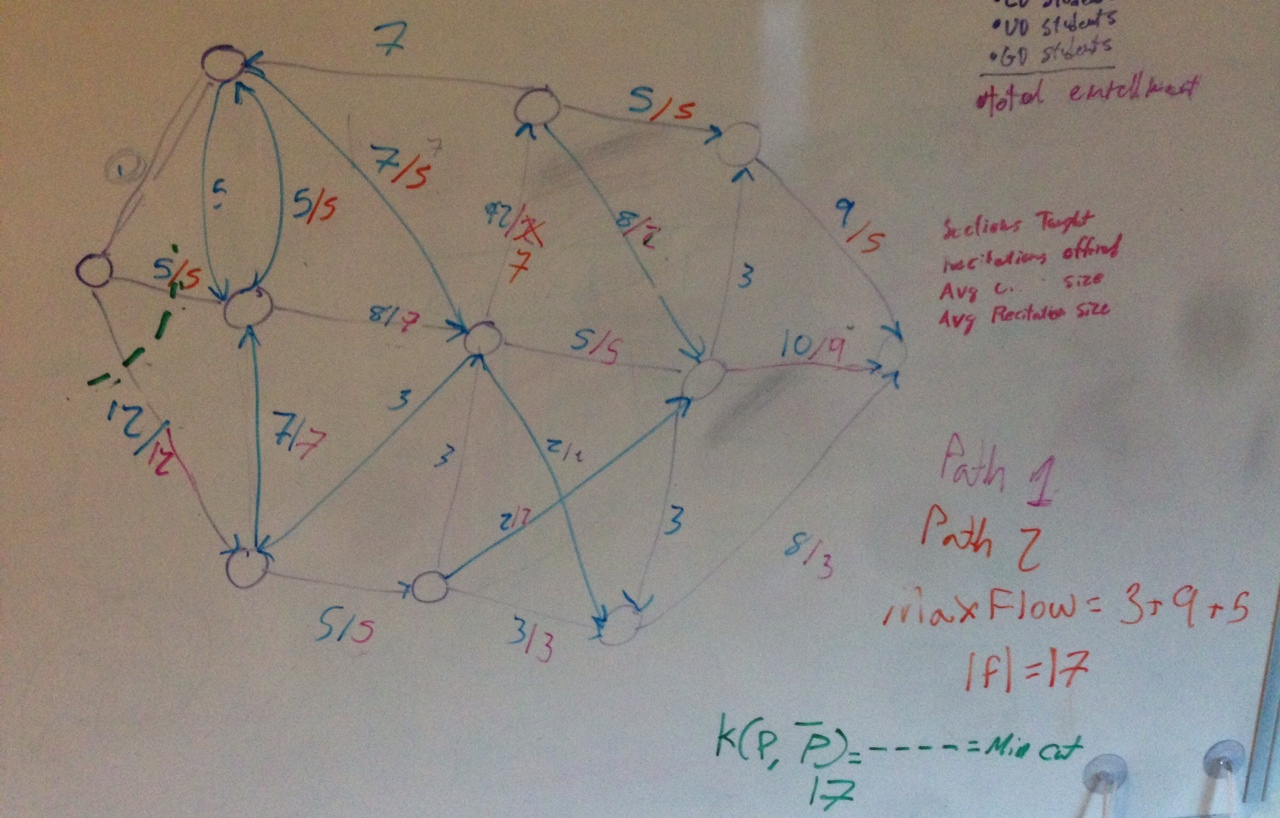
\includegraphics[width=100mm]{orig_flow.JPG}
\caption{Our original flow graph.}
\label{overflow}
\end{figure}
\\
\noindent{ \large b) The smallest capacity for X to increase water flow across the network would be 3. This is the maximum capacity that can be supported in terms of flow in our network. See Fig. 2 below for our new network.} 
\\
\begin{figure}[ht!]
\centering
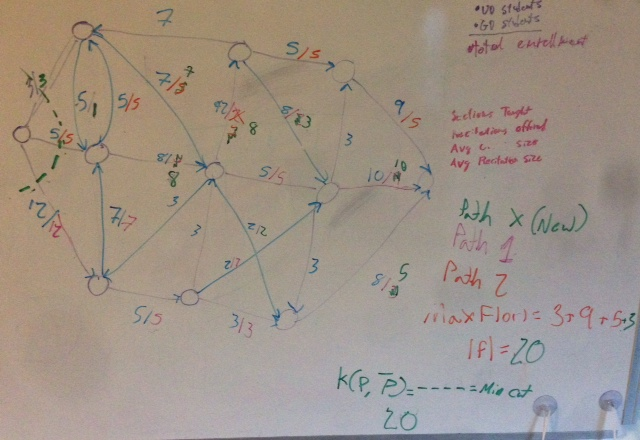
\includegraphics[width=100mm]{new_flow.JPG}
\caption{New modified flow graph with x = 3. }
\label{overflow}
\end{figure}
\\
\noindent{ \large c) The engineers can use the Ford-Fulkerson (FF) algorithm and the residual graph it produces to determine the max capacity of edge X. For problem B, we used the FF algorithm to discover that the maximum flow that can be pushed through X is 3. Anything greater than 3 can't be dealt with properly by the system and we get bottlenecking in the middle of the network. If we have graph G, the capacity of proposed Edge (u,v) is the max capacity of our our current graph ($M$) subtracted from the max capacity of our augmented graph ($M'$) i.e. $X = M' - M$ } 
\\

\noindent{\Large \bf Problem 2}
\\
\indent{\large We define $T$ to be a spanning tree of $G$. Let $w(T)=	\sum_{(x,y)\in T}$, and $w'(T)=w(T)-k$. We then consider a second spanning tree, $T'$, such that $w(T) \le w(T')$. If $(x,y)\notin T'$, then $w'(T')=w(T')\ge w'(T)$. Also, if $(x,y) \in T'$, then $w'(T')=w(T')-k \ge w(T)-k$. Either way, $w'(T) \le w'(T')$, so even if we reduce the weight of one of the edges in spanning tree $T$, it will still be a MST.}
\\
\\

\noindent{\Large \bf Problem 3}
\\
\indent{\large a) A sub-optimal, greedy approach to this problem would be to order all of the bids from largest to smallest in an array. Then going through the array, add every bid that does not have any over lap with a previous bid. So, to do this,we will initialize two arrays. In the first array we will put all of the bids sorted from largest to smallest. Then we will loop through the array, check if there is a land overlap, and if not we will add it to the second array, which is filled with bids we will accept. If there is a land overlap, we will skip the bid and move on to the next element in the array. The problem with this greedy algorithm is that it will not take into account the price per unit of land. This means we will blindly accept the biggest number, but we will not account for how much land the bidders are actually taking. In the example below, the brackets are the property line, and the numbers with dashes are the bids for the amount of land they want. Our algorithm would sort all of the bids and take the biggest ones first. So we would take the two tens, then the $5$, then the two $1$'s. This means our total profit would be $27$, in the first scenario. As we can see, the optimal solution would be to take the first $1$, then $10$, then the $5$ on the bottom, then the $9$, and finally the last $5$ to get a total profit of $30$.
\begin{verbatim}
  { [1][---10-----][1][--5--][---10-----]-- }
  { [--5--][--5--][--5--][----9----][--5--] }
\end{verbatim}
}

\indent{\large b) The correct way to solve this problem, would be to order all of the bids by their left end, such that $L_1\le L_2\le ... \le L_n$. We recurse on this ordered array of bids such that if we accept bid $i$, then our maximum total profit is $w(x_i)$, where $x_i$ is the $i^{th}$ bid, plus the maximum profit of from the subset of bids to the right of $x_i$. If we reject $x_i$, then our total maximum profit is the maximum profit from the subset of bids to the right of $x_i$, which is the set $\{x_{i+1},...,x_n\}$. In the following algorithm, $totalProfit$ is an integer that keeps track of the amount of profit from the accepted bids. The array $orderBids$ is an array of integers, where $orderBids.get(i)$, gets the amount of money offered by the $i^{th}$ bid. This algorithm will have a running time of $O(n*log(n))$, because while we are recursing through the list $O(n^2)$ times, we are deleting elements in the list as we go along.
\pagebreak
\begin{verbatim}
findMaxProfit(orderBids, totalProfit, i){
  if(orderBids.get(i) is empty){
    return totalProfit
  }
  totalProfit += (orderBids.get(i) + findMaxProfit(orderBids, totalProfit, i++))
  if(totalProfit >= findMaxProfit(orderBids, acceptedBids, i++)){
    orderBids.remove(i)
    return totalProfit
  }
  else{
    totalProfit -= orderBids.get(i)
    orderBids.remove(i)
    return findMaxProfit(orderBids, totalProfit, i++) 
  }  
}
main{
  totalProfit= 0
  orderBids = orderBidsbyLeft(Bids) //takes the bids we are given and orders them by left
  findMaxProfit(orderBids, totalProfit, 0)
}
\end{verbatim}
}
\noindent{\Large \bf Problem 4}
\\
\indent{\large To find a solution to solve this dilemma of uncooperative hobbits, we need to break it into two sub-problems. Problem a involves transforming our given graph into a flow diagram. Problem b requires us to run analysis on this flow to determine if it is possible for the hobbits to each reach the market while abiding by the rules given to us.}
\\
\indent(\large a) Because we know that the hobbits can never travel on the same path together, we can make each path have a maximum capacity of 1. This satisfies the requirement of only a single hobbit being on a path at once. We can see a transformation of a normal graph to our flow diagram in Figure 3 below. We know automatically for our new transformed graph that there has to be two edges out of $s$, and that there are two edges going to $t$. To find whether or not the paths in the middle are sufficient,we continue to part b, below. 
\\
\begin{figure}[ht!]
\centering
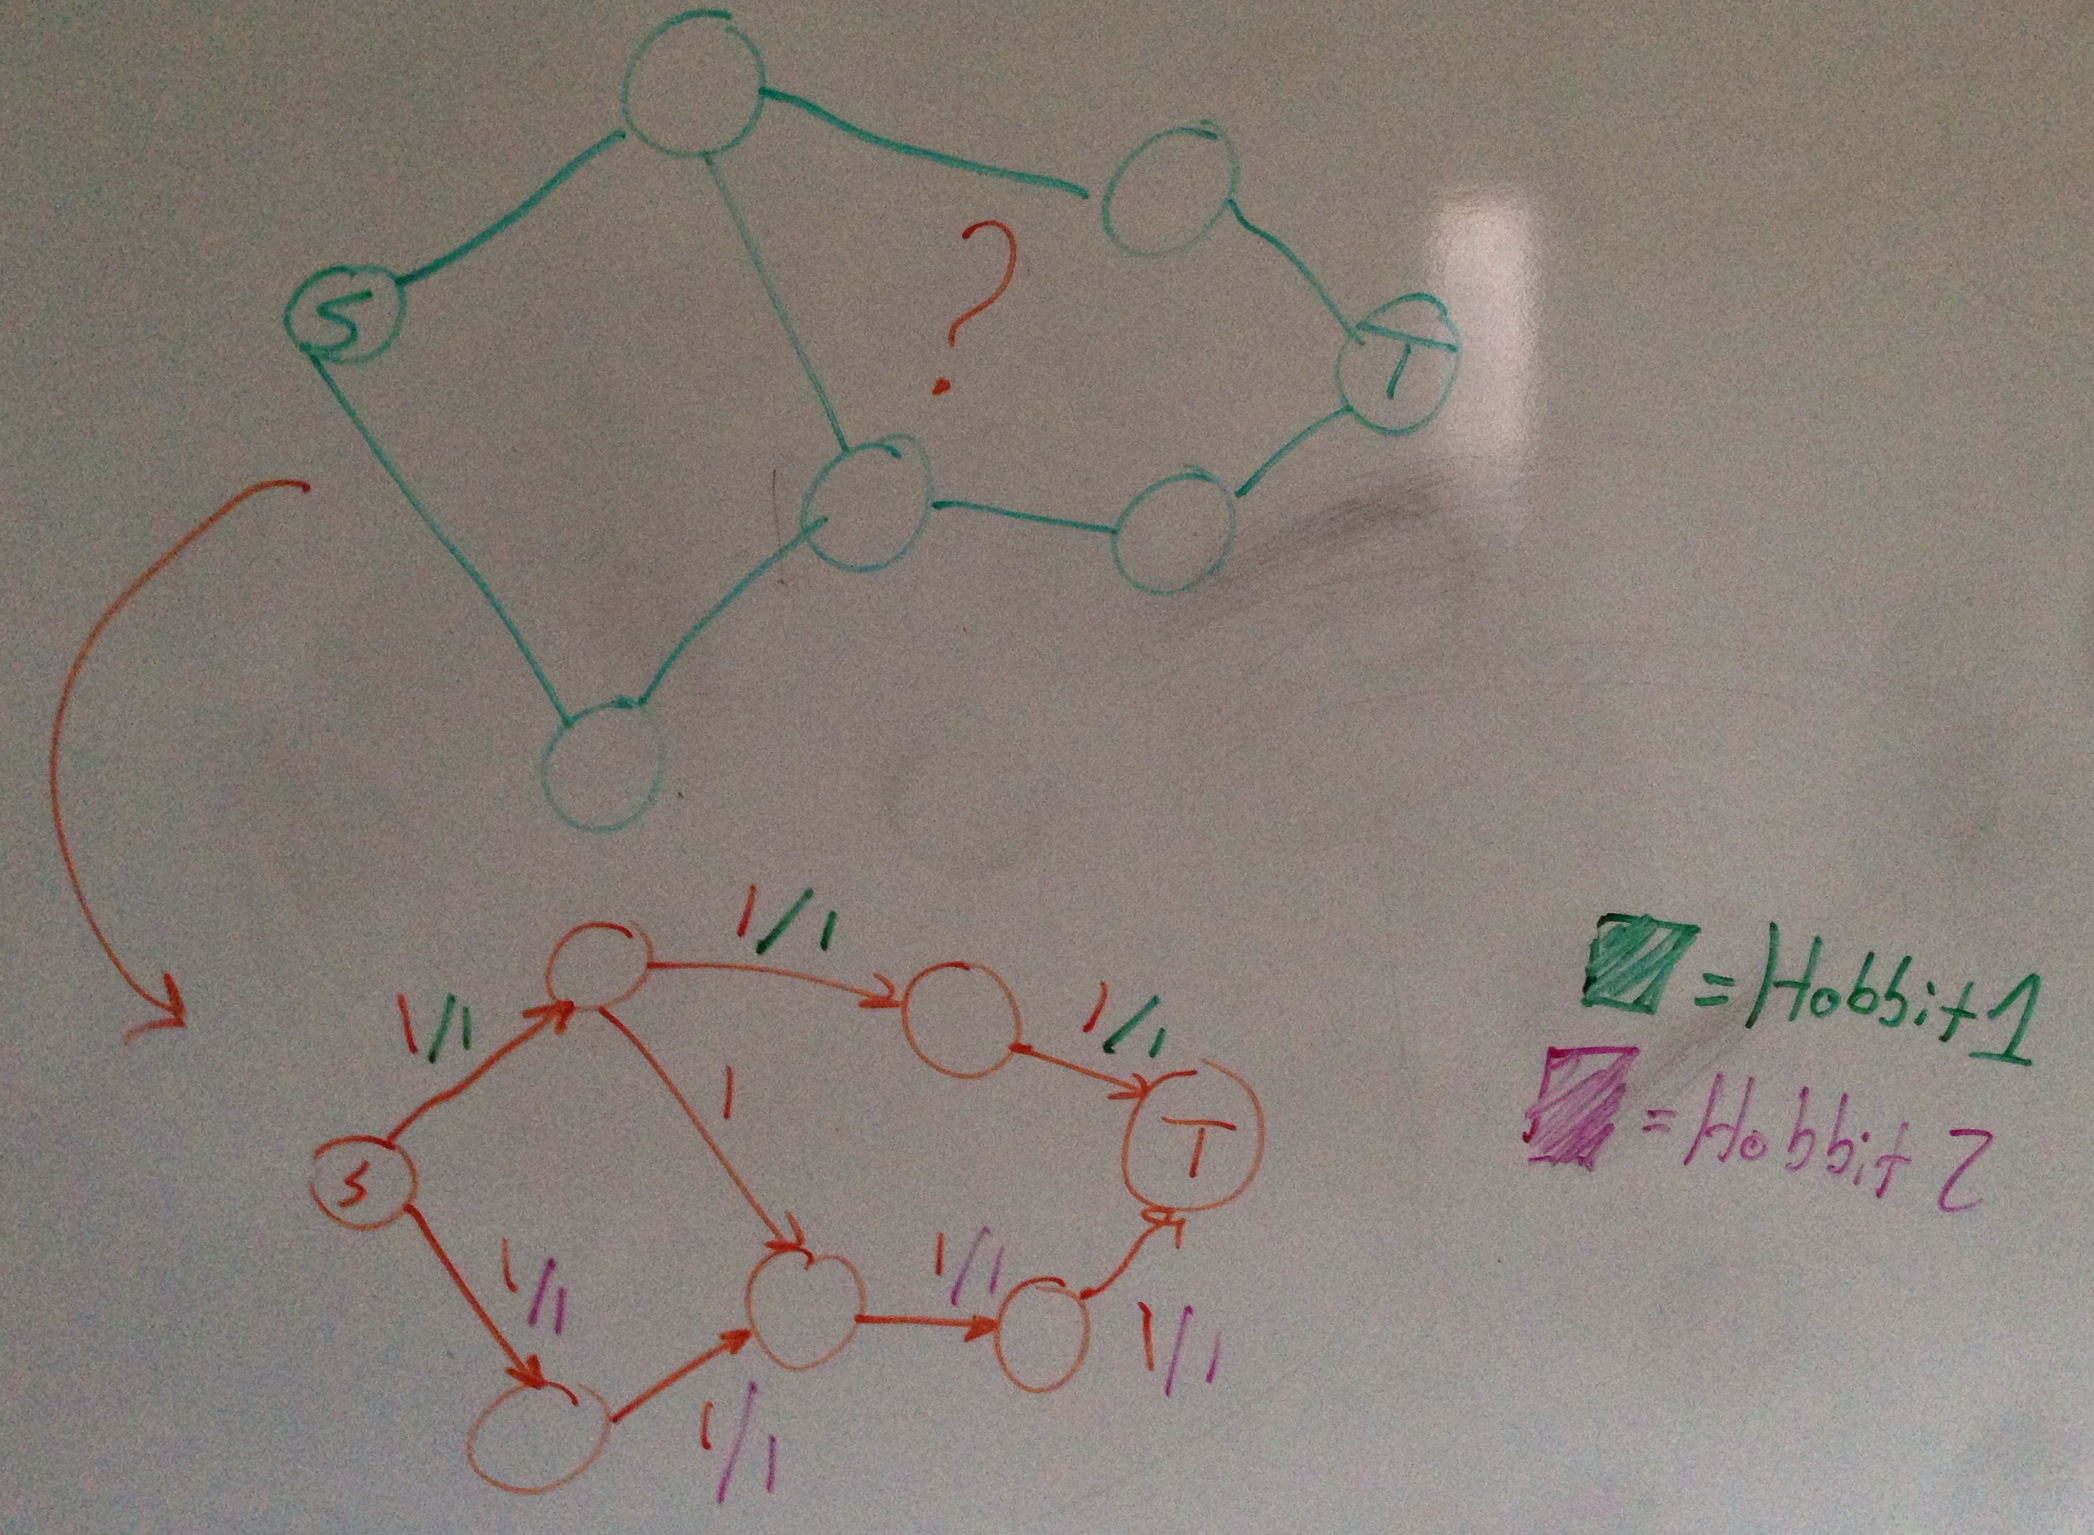
\includegraphics[width=107mm]{prob_4.JPG}
\caption{Transforming Graph and finding proper flow paths. }
\label{overflow}
\end{figure}
\\
\indent{\large b) Once we have our graph converted it is simply a matter of running the Ford-Fulkerson algorithm for max-flow to find the proper path for the hobbits to take given the restrictions, our max flow. Look at Figure 3 to see how we ran the FF algorithm on our two flows to find the possible paths for the hobbits. 
\\
\\
\noindent{\Large \bf Problem 5}
\\
\indent{\large To solve the poisoned wine problem, we need to give each of the bottles a serial number in binary. Bottle 1 (B1) would be given the label (1), Bottle 2 would have the label (10) with Bottle 12 having the label (1100), etc. Each rat is labelled with a bit, and they only sip from the wine that uses their bit. So in the case of Rat 1, he only drinks from wines with the first bit activated (1001,0011,101,...1). Rat 2, attached to the second bit, will only drink from bottles with the second bit activated (11,101010, 11010,...). If, in our case, a bottle is poisoned, we can see the chain of rats with each dead rat representing a bit of our poisoned bottle's serial number. If rats 1,2,4 die, we know that the number of our bad bottle is (1011) or Bottle 11. For n bottles, we need o$(lg(n))$ rats. See the table below for a sample of 4 rats with 15 bottles of wine, including a poisoned bottle 6. By finding that Rats 2 and 3 are dead, we know that bottle (0110) is poisoned. This is the bottle 6 that we expected. 
\\ 
\\
\centerline{\begin{tabular}{| l | c | r |}
  \hline                       
  Rat (Bit) & Bottles Consumed & Dead \\\hline
  1(0001) & 1,3,5,7,9,11,13,15 & N \\
  2(0010) & 2,3,6,7,10,11,14,15 & Y \\
  3(0100) & 4,5,6,7,12,13,14,15 & Y \\
  4(1000) & 8,9,10,11,12,13,14,15 & N \\
  \hline  
\end{tabular}}
\\
\newline
\noindent{ \Large \bf Sources}
\\
\noindent{$\bullet$ https://www.cs.princeton.edu/courses/archive/spring13/cos423/lectures/07NetworkFlowI-2x2.pdf}
%USEFUL FOR FLOWS%
\\

\end{document}